\section{Methods}

% Experiments build upon Sabatelli et al.
Much of the experiments and analysis discussed below, builds upon the work done in \citeauthor{sabatelli2018deep} (\citeyear{sabatelli2018deep}). This paper investigated TL properties of CNNs in the art classification domain. The main focus was on a comparison between CNN architectures pre-trained on ImageNet1K when they were either used as OTS feature extractors, or fine-tuned to the new task. It was suggested that FT resulted in substantially better performance than either training from scratch or using an OTS learning scheme.

\subsection{Dataset} \label{methods:dataset}

\begin{table*}[tb]
\centering
\small
\begin{tabular}{lllll}
\hline
\textbf{Task} & \textbf{\# Samples} & \textbf{\# Classes} & \textbf{Gini coefficient} & \textbf{Sample overlap} \\ \hline
Type classification & 9607 (77628) & 30 (801) & 0.466 (0.974) & 0.686 \\
Material classification & 7788 (96583) & 30 (136) & 0.563 (0.980) & 0.798 \\
Artist classification & 6530 (38296) & 30 (8592) & 0.236 (0.676) & 1 \\
Scaling experiment & 7926 (77628) & 15 (801) & 0.300 (0.974) & - \\ \hline
\end{tabular}
\caption{Overview of the used datasets. Values between brackets show the situation before balancing operations were performed. `Sample overlap' gives the average overlap between 2 of the 5 randomly generated sets per task ($i$ and $j$ where $i \neq j$).}
\label{methods:datasets}
\end{table*}

\begin{figure*}[bt]
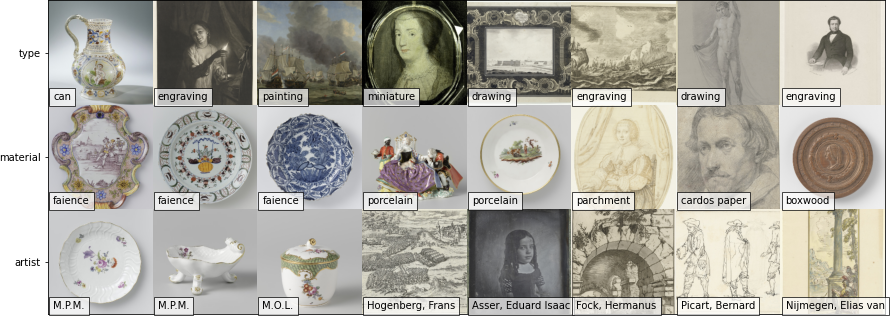
\includegraphics[width=\textwidth]{img/examples.png}
\caption{Example images from the \textit{Rijksmuseum Challenge}. Each row depicts a different task.}
\label{methods:eg}
\end{figure*}

Similar to \citeauthor{sabatelli2018deep}, used models are pre-trained on ImageNet1K, while the \textit{Rijksmuseum Challenge} dataset \citep{mensink14icmr} is used for the target tasks. This dataset consists of a large collection of digitized artworks, together with xml-formatted metadata. The classification tasks extracted from it are: (1) \textit{Type classification}, containing labels as `painting', `sculpture', `drawing', etc.; (2) \textit{Material classification}, with labels as `paper', `porcelain', `silver', etc.; and finally, (3) \textit{Artist classification}, where the model has to predict who the creator is. Figure \ref{methods:eg} shows labelled examples for all three tasks.

The full dataset contains 112,039 images, and allows for multiple or zero labels per classification task. Samples are excluded from a task if they contain no labels for it. Samples containing more than one label are excluded as well, since analysis showed that in all cases this is true for only a small portion of the dataset.% Note that this last point is different from \citeauthor{sabatelli2018deep}, which took the first occurring class in these cases.

There are still many samples and classes left after doing the operations described above. Samples are also unevenly distributed among classes, with Gini-coefficients being as high as 0.98\footnote{The Gini-coefficient is a measure of balance, with 0 meaning all classes have the same number of samples, and 1 meaning all samples belong to a single class. A uniform distribution has coefficient $\frac{1}{3}$}. To counteract this, only the 30 most occurring classes are selected, and a cap of 1000 instances per class is enforced by taking a random sample when this limit is exceeded. Table \ref{methods:datasets} shows the result of these balancing and subsampling operations. The situation prior is shown between brackets.

It is worth noting that \citeauthor{sabatelli2018deep} does not perform these operations. They are performed here, because the current study is interested in small datasets specifically.

All datasets are split up into 80\%, 10\%, 10\% training, validating and testing sets. For robustness, five subsets are randomly generated per classification task, such that each experiment can be run five times. The average sample overlap between two of the five datasets is shown in table \ref{methods:datasets} as well.

Besides the tasks described above, table \ref{methods:datasets} shows an experiment called \textit{Scaling}. The goal of this experiment is to see how the findings of this paper hold up as dataset sizes are gradually shrunk. It does this by taking the top 15 classes of type classification, and scaling it 4 times by a factor $\sqrt[4]{\frac{1}{10}} \approx 0.56$. The 5 datasets produced in this manner are then respectively 100\%, 56\%, 32\%, 18\% and 10\% the size of the dataset shown in table \ref{methods:datasets}. Steps are taken to ensure the distribution remains the same. Finally, also here 5 datasets are generated per scaling factor, leading to a total of 25 datasets. The same 80\%, 10\%, 10\% split is used for all.

% Mention the challenges and show the table, of course. Also add max and min classes per category to the table maybe
% Don't forget to tell that images get scaled and cropped to 224 * 224 size and imagenet normalised
% Dataset described in more detail in Appendix A, including histograms and confusion matrices + balancing 'algorithm'

\subsection{Models} \label{methods:models}
Eight different neural network architectures are used throughout this paper, of which four are CNN-based and four VT-based. When multiple versions are available (i.e. `base', `small', `tiny'), `base'/`medium' ones are chosen.

To start off with CNNs, \texttt{ResNet50} \citep{he2016deep} and \texttt{VGG19} \citep{simonyan2014very} are chosen, as these were the best performing models in \citeauthor{sabatelli2018deep} for respectively FT and OTS TL. In addition, \citeauthor{matsoukas2021time} (\citeyear{matsoukas2021time}) used \texttt{ResNet50} too, while \citeauthor{zhou2021convnets} (\citeyear{zhou2021convnets}) used \texttt{ResNet101} and \texttt{ResNet152}. To also add some more recent CNNs, \texttt{ConvNext} \citep{liu2022convnet} -- a purely CNN-based model inspired by VTs' recent success -- and \texttt{EfficientNetV2} \citep{tan2021efficientnetv2} are included.

For VTs, versions with a 16x16 patch size are chosen. The first model is the original VT \citep{dosovitskiy2020image}, which will be referred to as \texttt{ViT}. Next is \texttt{Swin} \citep{liu2021swin}, because it showed promising performance in \citeauthor{zhou2021convnets}. The final two are \texttt{DeiT} and \texttt{BeiT}. The small version of \texttt{DeiT} was used in \citeauthor{matsoukas2021time} (\citeyear{matsoukas2021time}), because it is similar in size to \texttt{ResNet50}, to which it was compared. In this work, however, also a base-sized version is chosen. Specifically, the version that does not include output for distillation learning.

% Section \ref{related_work} mentioned DeiT \citep{touvron2021training} too, as the distillation based architecture. The small version of this architecture was used in \citeauthor{matsoukas2021time} (\citeyear{matsoukas2021time}), since it is similar in size to ResNet50, to which it was compared. Here, however, a base-sized version is chosen. Specifically, the version that does not include output for distillation learning.
% TODO TODO TODO TODO TODO TODO TODO TODO YOU FORGOT TO MENTION BEIT!!!
% TODO 2: im not completely happy with the part about DeiT. Doesn't flow super nicely

All VT-based models have a bit over 86 million parameters. \texttt{ConvNext} is of similar size, with 88.6 million parameters. \texttt{ResNet50} and \texttt{EfficientNetV2} are smaller, with 25.6 and 13.6 million, respectively, while \texttt{VGG19} is the largest model, with 143.7 million parameters. It should be mentioned that for both OTS TL and FT, preliminary experiments were performed with `small' and `tiny' models. The results of these suggested that similar conclusions could have been drawn if these were used instead.

% General information (4 per type, base/tiny etc)
% Paragraph/section about CNN models
%  - ResNet50 and VGG19 best fine-tuned and ots networks in Sabatelli
%  - ResNet50 I think also used in medical imaging paper; ResNet101 ots vt paper
%  * Convnext and EfficientNetV2 to have some more modern ones in the mix (to make comparison more fair)
% Paragraph/section about VT models -- explain the idea behind each in 1 sentence maybe (also for CNNs)

\subsection{Hyperparameters and data augmentation}
All images are resized to a $224 \times 224$ resolution. This is achieved by first scaling them to the desired size along the shortest axis (retaining aspect ratio), and then taking a center crop along the longer axis. In addition, all images are normalized to the RGB mean and standard deviation of ImageNet1K.

For all models, the linear classification layer is replaced as to fit the new task. Cross entropy loss uses the raw outputs of this layer (conform \texttt{PyTorch} documentation), together with one-hot encoded prediction targets. An early stop occurs after 10 epochs without improved loss on the validation set, and the model with the lowest loss is benchmarked on the testing set.

For OTS TL, the Adam optimizer is used with standard \texttt{PyTorch} parameters (\texttt{lr}=1e-3, $\beta_1=0.9$, $\beta_2=0.999$), and a batch size of 256. For FT, more is needed to achieve good convergence, especially for VT-based architectures. Used hyperparameters, etc. are partially inspired by \citeauthor{matsoukas2021time} (\citeyear{matsoukas2021time}) and \citeauthor{zhou2021convnets} (\citeyear{zhou2021convnets}). The Adam learning rate now starts off at 1e-4, and is reduced by a factor 10 after 3 epochs without improvement (i.e. patience=2); the batch size is reduced to 32; label smoothing of 0.1 is added to the cross entropy loss, and a dropout layer with p=0.2 is inserted before the classification layer. Finally, input images are augmented with random horizontal flips and rotations in a $\pm 10 ^\circ$ range.

\subsection{Hardware and software}
All experiments are conducted on a single compute node containing one 32 GB Nvidia V100 GPU. These nodes are constituents of the \textit{Peregrine high performance computing cluster}, belonging to the \textit{University of Groningen's Center for Information Technology}. The FT experiments take advantage of the V100's mixed precision acceleration. An exception is made for the type classification experiment, as this one is also used to compare OTS TL and FT in terms of time/accuracy trade-offs. Preliminary findings suggested that using mixed precision does not affect performance for the aforementioned experiments, however.

The \texttt{PyTorch} machine learning framework is used, and many pre-trained models are taken from its \texttt{Torchvision} library. Exceptions are \texttt{EfficientNetV2}, \texttt{Swin}, \texttt{DeiT} and \texttt{BeiT}, which are taken from the \texttt{Timm} library\footnote{\url{https://timm.fast.ai/}.}.

Finally, all source code and data will be made available on GitHub\footnote{\url{https://github.com/IndoorAdventurer/ViTTransferLearningForArtClassification}.}.

